\documentclass[aspectratio=169]{beamer}
\usepackage{tikz}
\usepackage{amsmath}
\usetikzlibrary{shapes.geometric, arrows.meta, positioning, fit, calc, backgrounds}

% Colors: Background white, text blue
\setbeamercolor{background canvas}{bg=white}
\setbeamercolor{normal text}{fg=blue!80!black}
\setbeamercolor{title}{fg=blue!80!black}
\setbeamercolor{frametitle}{fg=blue!80!black}
\setbeamercolor{structure}{fg=blue!80!black}
\setbeamercolor{item}{fg=blue!80!black}
\setbeamercolor{itemize item}{fg=blue!80!black}
\setbeamercolor{itemize subitem}{fg=blue!80!black}

% TikZ styles
\tikzset{
    box/.style={draw=blue!80!black, thick, fill=white, rounded corners, align=center, text=blue!80!black, minimum height=0.8cm},
    arrow/.style={-Latex, thick, blue!80!black},
    dasharrow/.style={-Latex, dashed, thick, blue!80!black}
}

\title{\textbf{Attention-Aware Study Assistant}}
\subtitle{GenAI System Building Challenge}
\author{Microservices Architecture Presentation}
\date{}

\begin{document}

\begin{frame}
    \titlepage
\end{frame}

% 1. Brief description of what the system does
\begin{frame}{System Overview}
    \begin{itemize}
        \item \textbf{What it is:} A cloud-native, GenAI-powered NLP educational system built with 10 microservices.
        \item \textbf{Core Function:} Monitors a learner's cognitive state in real-time and dynamically adapts educational content delivery based on cognitive fatigue signals.
        \item \textbf{Modes of Operation:}
        \begin{itemize}
            \item \textbf{Learning Mode:} Video-based learning. Fatigue is inferred from player interactions (seek, pause, speed changes).
            \item \textbf{Quiz Mode:} Text-based Q\&A. Fatigue is inferred from keypress dynamics and response latency.
        \end{itemize}
    \end{itemize}
\end{frame}

% 2. How the system uses ReAct agentic loop
\begin{frame}{ReAct Agentic Loop}
    The system implements a \textbf{ReAct (Reason + Act)} loop where each interaction triggers a 4-step cognitive process:
    \vspace{0.3cm}
    \begin{center}
    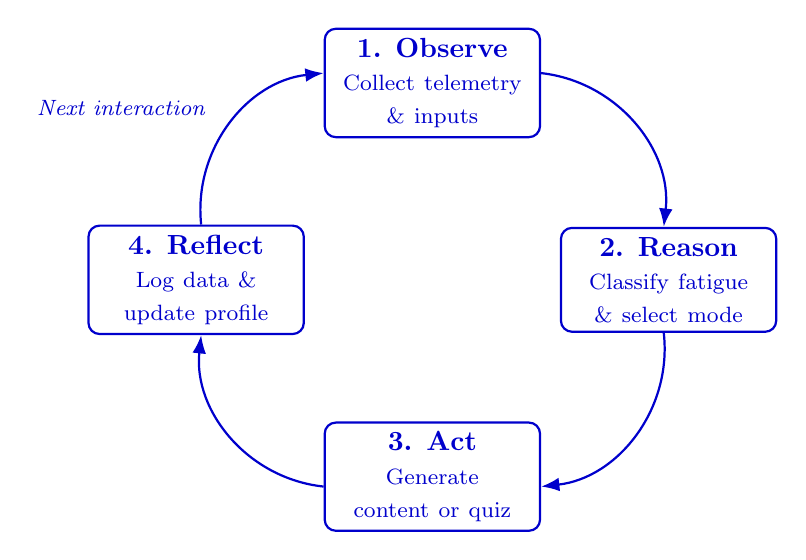
\begin{tikzpicture}[auto, thick]
        % Define nodes in a circle
        \node [box, text width=2.5cm] (obs) at (90:2.5cm) {\textbf{1. Observe}\\ \footnotesize Collect telemetry \& inputs};
        \node [box, text width=2.5cm] (reason) at (0:3cm) {\textbf{2. Reason}\\ \footnotesize Classify fatigue \& select mode};
        \node [box, text width=2.5cm] (act) at (270:2.5cm) {\textbf{3. Act}\\ \footnotesize Generate content or quiz};
        \node [box, text width=2.5cm] (reflect) at (180:3cm) {\textbf{4. Reflect}\\ \footnotesize Log data \& update profile};

        \draw [arrow] (obs) to[bend left=45] (reason);
        \draw [arrow] (reason) to[bend left=45] (act);
        \draw [arrow] (act) to[bend left=45] (reflect);
        \draw [arrow] (reflect) to[bend left=45] node[midway, left, font=\footnotesize\itshape, xshift=-0.2cm, yshift=0.2cm] {Next interaction} (obs);
    \end{tikzpicture}
    \end{center}
\end{frame}

% 3. Diagram showing the microservices architecture
\begin{frame}{Microservices Architecture}
    \begin{center}
    \resizebox{\textwidth}{!}{
    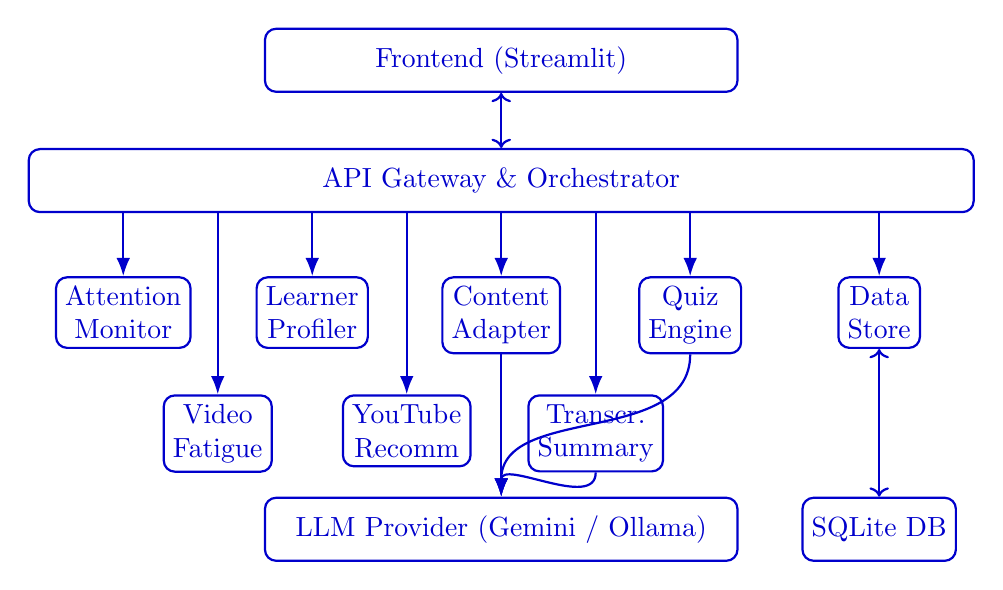
\begin{tikzpicture}[node distance=1cm, auto]
        \node [box, minimum width=6cm] (fe) {Frontend (Streamlit)};
        \node [box, minimum width=12cm, below=0.7cm of fe] (gw) {API Gateway \& Orchestrator};
        \draw [arrow, <->] (fe) -- (gw);
        
        % Row 1
        \node [box, below=0.8cm of gw, xshift=-4.8cm] (s1) {Attention\\Monitor};
        \node [box, below=0.8cm of gw, xshift=-2.4cm] (s2) {Learner\\Profiler};
        \node [box, below=0.8cm of gw, xshift=0cm] (s3) {Content\\Adapter};
        \node [box, below=0.8cm of gw, xshift=2.4cm] (s4) {Quiz\\Engine};
        \node [box, below=0.8cm of gw, xshift=4.8cm] (s6) {Data\\Store};

        % Row 2 (offset to sit in the gaps)
        \node [box, below=2.3cm of gw, xshift=-3.6cm] (s8) {Video\\Fatigue};
        \node [box, below=2.3cm of gw, xshift=-1.2cm] (s9) {YouTube\\Recomm};
        \node [box, below=2.3cm of gw, xshift=1.2cm] (s10) {Transcr.\\Summary};
        
        \draw [arrow] (gw.south -| s1.north) -- (s1.north);
        \draw [arrow] (gw.south -| s2.north) -- (s2.north);
        \draw [arrow] (gw.south -| s3.north) -- (s3.north);
        \draw [arrow] (gw.south -| s4.north) -- (s4.north);
        \draw [arrow] (gw.south -| s6.north) -- (s6.north);

        \draw [arrow] (gw.south -| s8.north) -- (s8.north);
        \draw [arrow] (gw.south -| s9.north) -- (s9.north);
        \draw [arrow] (gw.south -| s10.north) -- (s10.north);
        
        % DB and LLM
        \node [box, below=3.6cm of gw, xshift=4.8cm] (db) {SQLite DB};
        \node [box, below=3.6cm of gw, xshift=0cm, minimum width=6cm] (llm) {LLM Provider (Gemini / Ollama)};
        
        \draw [arrow, <->] (s6.south) -- (db.north);
        \draw [arrow] (s3.south) -- (llm.north);
        \draw [arrow] (s4.south) to[out=270, in=90] (llm.north);
        \draw [arrow] (s10.south) to[out=270, in=90] (llm.north);
    \end{tikzpicture}
    }
    \end{center}
\end{frame}

% 4. One slide each describing how each microservice acts.

\begin{frame}{Attention Monitor Agent}
    \begin{itemize}
        \item \textbf{Purpose:} Passive fatigue classifier tracking cognitive load in real-time.
        \item \textbf{Score Calculation:}
        \begin{equation*}
            S_{fatigue} = 0.4 \left( \frac{\sigma_{keypress}}{\mu_{baseline}} \right) + 0.3 \left( \min\left(1, \frac{t_{delay}}{t_{max}}\right) \right) + 0.3 ( 1 - S_{quiz\_trend} )
        \end{equation*}
        \item Weights: 40\% Keypress Variance, 30\% Response Delay, 30\% Quiz Trend.
    \end{itemize}
    \vspace{0.2cm}
    \begin{center}
    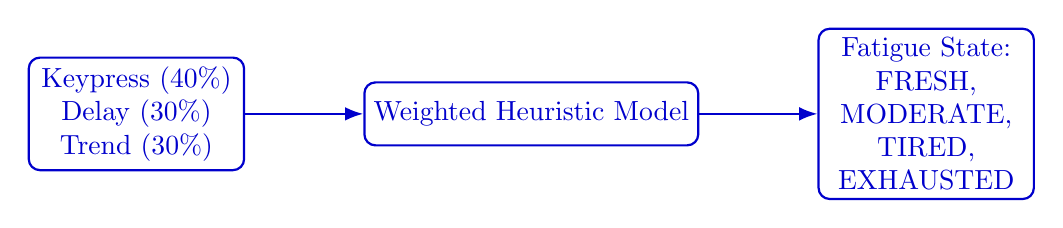
\begin{tikzpicture}[node distance=2cm]
        \node [box, text width=2.5cm] (inputs) {Keypress (40\%) \\ Delay (30\%) \\ Trend (30\%)};
        \node [box, right=1.5cm of inputs] (logic) {Weighted Heuristic Model};
        \node [box, right=1.5cm of logic, text width=2.5cm] (out) {Fatigue State: \\ FRESH, MODERATE, TIRED, EXHAUSTED};
        \draw [arrow] (inputs) -- (logic);
        \draw [arrow] (logic) -- (out);
    \end{tikzpicture}
    \end{center}
\end{frame}

\begin{frame}{Learner Profiler Agent}
    \begin{itemize}
        \item \textbf{Purpose:} Adaptive learner model maintenance over time.
        \item \textbf{Tracking:} Updates mastery score, difficulty level, and preferred mode based on continuous quiz performance and interaction history.
    \end{itemize}
    \vspace{0.2cm}
    \begin{center}
    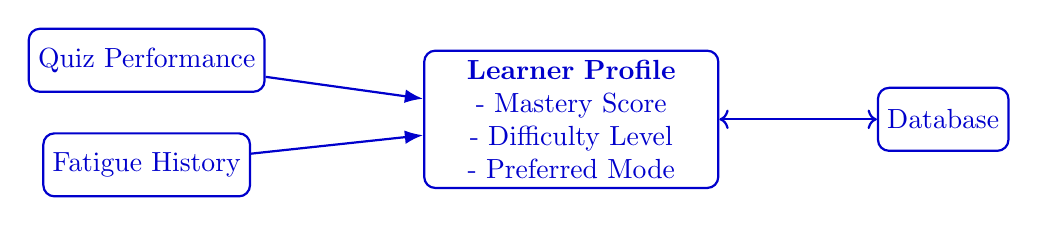
\begin{tikzpicture}[node distance=1.5cm]
        \node [box] (quiz) {Quiz Performance};
        \node [box, below=0.5cm of quiz] (fat) {Fatigue History};
        \node [box, right=2cm of quiz, yshift=-0.75cm, text width=3.5cm] (prof) {\textbf{Learner Profile}\\- Mastery Score\\- Difficulty Level\\- Preferred Mode};
        \node [box, right=2cm of prof] (db) {Database};
        \draw [arrow] (quiz) -- (prof);
        \draw [arrow] (fat) -- (prof);
        \draw [arrow, <->] (prof) -- (db);
    \end{tikzpicture}
    \end{center}
\end{frame}

\begin{frame}{Content Adaptation Agent}
    \begin{itemize}
        \item \textbf{Purpose:} Dynamically selects teaching modes based on fatigue.
    \end{itemize}
    \vspace{0.5cm}
    \begin{center}
    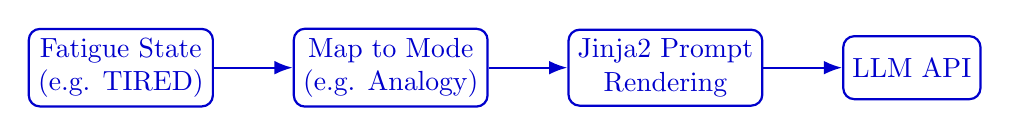
\begin{tikzpicture}[node distance=1.5cm]
        \node [box] (state) {Fatigue State \\ (e.g. TIRED)};
        \node [box, right=1cm of state] (map) {Map to Mode \\ (e.g. Analogy)};
        \node [box, right=1cm of map] (prompt) {Jinja2 Prompt \\ Rendering};
        \node [box, right=1cm of prompt] (llm) {LLM API};
        \draw [arrow] (state) -- (map);
        \draw [arrow] (map) -- (prompt);
        \draw [arrow] (prompt) -- (llm);
    \end{tikzpicture}
    \end{center}
\end{frame}

\begin{frame}{Quiz Engine}
    \begin{itemize}
        \item \textbf{Purpose:} Adaptive quiz generator \& evaluator.
        \item \textbf{LLM Abstraction:} Auto-routes requests to a Cloud API (Gemini) or a Local Fallback (Ollama) if offline or for privacy.
        \item \textbf{LLM-as-a-judge Scoring:} 
        \begin{equation*}
            S_{score} = \text{LLM\_Evaluate}(\text{Answer}) \in [0.0, 1.0]
        \end{equation*}
        Evaluates free-text answers on a scale from 0.0 to 1.0 based on semantic correctness, which dynamically updates the learner's mastery profile.
    \end{itemize}
    \vspace{0.2cm}
    \begin{center}
    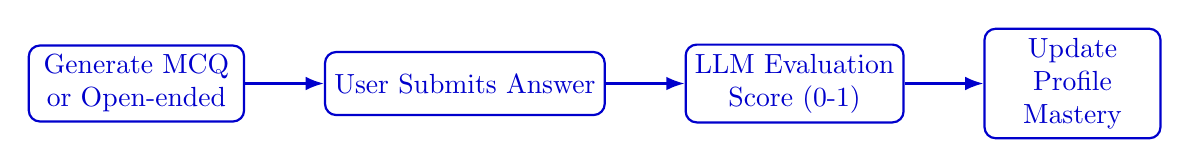
\begin{tikzpicture}[node distance=1.5cm]
        \node [box, text width=2.5cm] (gen) {Generate MCQ or Open-ended};
        \node [box, right=1cm of gen] (ans) {User Submits Answer};
        \node [box, right=1cm of ans] (eval) {LLM Evaluation \\ Score (0-1)};
        \node [box, right=1cm of eval, text width=2cm] (prof) {Update Profile Mastery};
        \draw [arrow] (gen) -- (ans);
        \draw [arrow] (ans) -- (eval);
        \draw [arrow] (eval) -- (prof);
    \end{tikzpicture}
    \end{center}
\end{frame}

\begin{frame}{Orchestrator}
    \begin{itemize}
        \item \textbf{Purpose:} Central ReAct agentic loop controller routing all traffic.
    \end{itemize}
    \vspace{0.5cm}
    \begin{center}
    
\begin{tikzpicture}[node distance=1.5cm]
        \node [box] (fe) {Frontend App};
        \node [box, right=2cm of fe] (orch) {\textbf{Orchestrator}\\ (FastAPI Gateway)};
        \node [box, right=2cm of orch] (svcs) {Microservices};
        \draw [arrow, <->] (fe) -- node[above, font=\footnotesize] {HTTP} (orch);
        \draw [arrow, <->] (orch) -- node[above, font=\footnotesize] {Internal API} (svcs);
    \end{tikzpicture}
    \end{center}
\end{frame}

\begin{frame}{Data Persistence Service}
    \begin{itemize}
        \item \textbf{Purpose:} Centralised storage and session export layer.
        \item \textbf{ORM (Object-Relational Mapping):} Abstracts raw SQL syntax by allowing us to interact with the database using Python objects/classes directly. This prevents SQL injection and provides a structured schema for our 5 tables.
    \end{itemize}
    \vspace{0.2cm}
    \begin{center}
    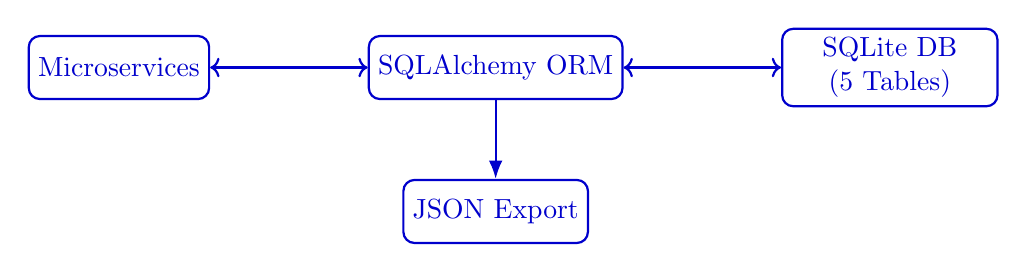
\begin{tikzpicture}[node distance=1.5cm]
        \node [box] (svcs) {Microservices};
        \node [box, right=2cm of svcs] (orm) {SQLAlchemy ORM};
        \node [box, right=2cm of orm, text width=2.5cm] (db) {SQLite DB\\(5 Tables)};
        \node [box, below=1cm of orm] (export) {JSON Export};
        \draw [arrow, <->] (svcs) -- (orm);
        \draw [arrow, <->] (orm) -- (db);
        \draw [arrow] (orm) -- (export);
    \end{tikzpicture}
    \end{center}
\end{frame}

\begin{frame}{Frontend Application}
    \begin{itemize}
        \item \textbf{Purpose:} Streamlit interactive user interface with dual modes.
    \end{itemize}
    \vspace{0.5cm}
    \begin{center}
    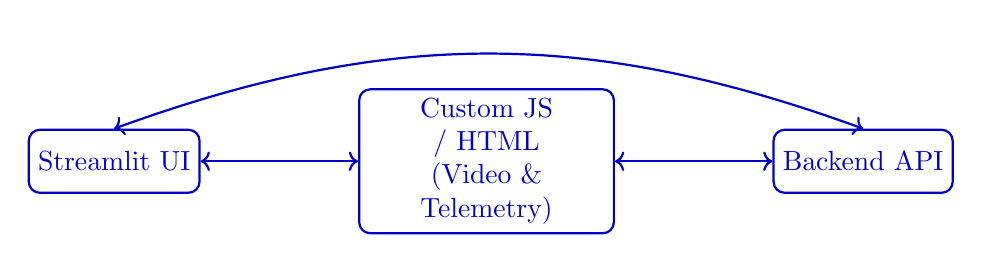
\begin{tikzpicture}[node distance=2cm]
        \node [box] (ui) {Streamlit UI};
        \node [box, right=2cm of ui, text width=3cm] (js) {Custom JS / HTML \\ (Video \& Telemetry)};
        \node [box, right=2cm of js] (api) {Backend API};
        \draw [arrow, <->] (ui) -- (js);
        \draw [arrow, <->] (js) -- (api);
        \draw [arrow, <->] (ui.north) to[bend left=20] (api.north);
    \end{tikzpicture}
    \end{center}
\end{frame}

\begin{frame}{Video Fatigue Monitor}
    \begin{itemize}
        \item \textbf{Purpose:} Maps player events to cognitive fatigue scores.
        \item \textbf{Score Calculation \& Decay Mechanic:} 
        \begin{equation*}
            F(t) = \sum_{i} \text{Impact}(E_i) \cdot e^{-\lambda (t - t_i)}
        \end{equation*}
        where $E_i$ are discrete events (e.g., Pause $= +0.08$) and $\lambda = 0.02$ represents the natural cognitive recovery rate over time.
        \item \textbf{Fatigue Updates:} Blends local UI tracking (80\%) with server-side computations (20\%) for smooth visuals.
    \end{itemize}
    \vspace{0.1cm}
    \begin{center}
    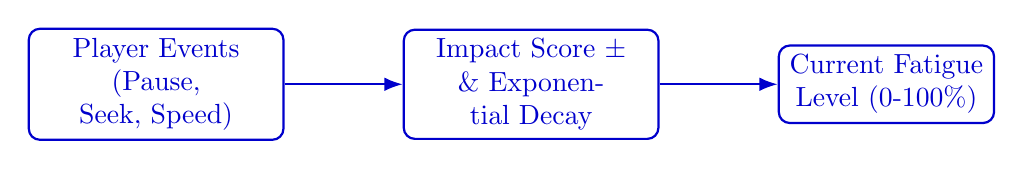
\begin{tikzpicture}[node distance=1.5cm]
        \node [box, text width=3cm] (events) {Player Events \\ (Pause, Seek, Speed)};
        \node [box, right=1.5cm of events, text width=3cm] (calc) {Impact Score $\pm$ \\ \& Exponential Decay};
        \node [box, right=1.5cm of calc, text width=2.5cm] (score) {Current Fatigue \\ Level (0-100\%)};
        \draw [arrow] (events) -- (calc);
        \draw [arrow] (calc) -- (score);
    \end{tikzpicture}
    \end{center}
\end{frame}

\begin{frame}{YouTube Recommender}
    \begin{itemize}
        \item \textbf{Purpose:} Fetches and ranks topic-relevant educational videos.
    \end{itemize}
    \vspace{0.5cm}
    \begin{center}
    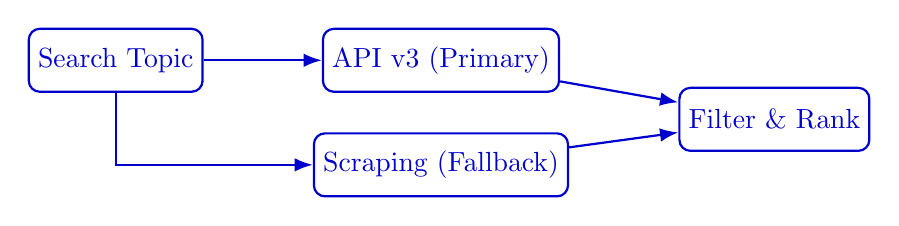
\begin{tikzpicture}[node distance=1.5cm]
        \node [box] (query) {Search Topic};
        \node [box, right=1.5cm of query] (api) {API v3 (Primary)};
        \node [box, below=0.5cm of api] (scrape) {Scraping (Fallback)};
        \node [box, right=1.5cm of api, yshift=-0.75cm] (filter) {Filter \& Rank};
        \draw [arrow] (query) -- (api);
        \draw [arrow] (query) |- (scrape);
        \draw [arrow] (api) -- (filter);
        \draw [arrow] (scrape) -- (filter);
    \end{tikzpicture}
    \end{center}
\end{frame}

\begin{frame}{Transcription Summary Agent}
    \begin{itemize}
        \item \textbf{Purpose:} Generates learner-friendly video summaries.
        \item \textbf{Trigger Threshold (0.75):} Intervenes precisely before cognitive exhaustion ($\ge 75\%$).
        \item \textbf{Pomodoro Dynamics:} A time-management method recognizing that human focus naturally wanes after $\sim$25 minutes. This system models that peak cognitive limit, triggering a summary break just as attention starts to sharply decline to preserve learning flow.
    \end{itemize}
    \vspace{0.1cm}
    \begin{center}
    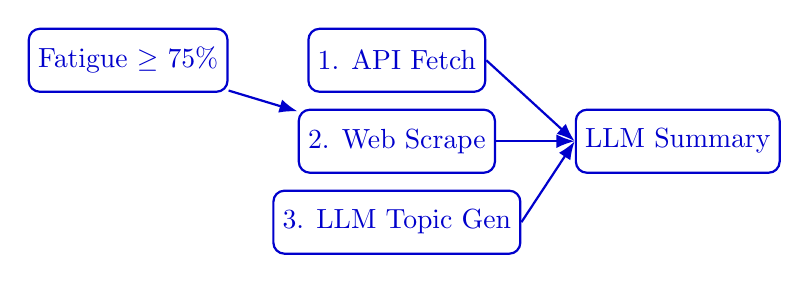
\begin{tikzpicture}[node distance=1cm]
        \node [box] (trigger) {Fatigue $\ge$ 75\%};
        \node [box, right=1cm of trigger] (t1) {1. API Fetch};
        \node [box, below=0.2cm of t1] (t2) {2. Web Scrape};
        \node [box, below=0.2cm of t2] (t3) {3. LLM Topic Gen};
        \node [box, right=1cm of t2] (llm) {LLM Summary};
        \draw [arrow] (trigger) -- (t2);
        \draw [arrow] (t1.east) -- (llm.west);
        \draw [arrow] (t2.east) -- (llm.west);
        \draw [arrow] (t3.east) -- (llm.west);
    \end{tikzpicture}
    \end{center}
\end{frame}

\begin{frame}{Future Work}
    \begin{itemize}
        \item \textbf{Adaptable Video Generation:} Dynamically generating or editing video content to match learner states. (e.g., leveraging research from SaralAI on explaining research papers via video).
        \item \textbf{Advanced Cognitive Models:} Scaling to more accurate machine learning algorithms for determining cognitive states beyond heuristics.
        \item \textbf{Multi-modal Biometrics:} Integrating webcam-based eye-tracking and facial expression analysis for richer, passive fatigue detection.
        \item \textbf{Curriculum Integration:} Expanding beyond isolated topics to map knowledge gaps across a full semester's curriculum.
    \end{itemize}
\end{frame}

\begin{frame}{Cloud Deployment Strategy}
    \begin{itemize}
        \item \textbf{Streamlit Cloud (Frontend):} Native, zero-config hosting for Streamlit; auto-deploys via GitHub.
        \item \textbf{Render.com (Backend API):} PaaS that natively supports FastAPI, offering managed persistent disks for SQLite and effortless horizontal scaling for our 10 microservices.
    \end{itemize}
    \vspace{0.4cm}
    \begin{center}
    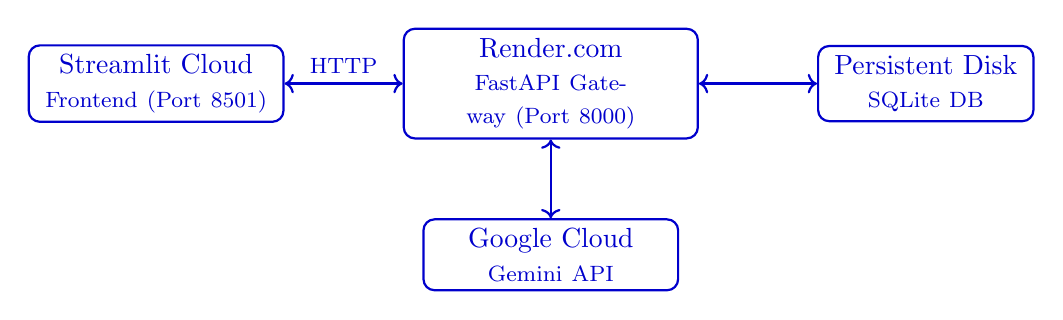
\begin{tikzpicture}[node distance=1.5cm]
        \node [box, text width=3cm] (fe) {Streamlit Cloud \\ \footnotesize Frontend (Port 8501)};
        \node [box, right=1.5cm of fe, text width=3.5cm] (be) {Render.com \\ \footnotesize FastAPI Gateway (Port 8000)};
        \node [box, right=1.5cm of be, text width=2.5cm] (db) {Persistent Disk \\ \footnotesize SQLite DB};
        \node [box, below=1cm of be, text width=3cm] (llm) {Google Cloud \\ \footnotesize Gemini API};
        
        \draw [arrow, <->] (fe) -- node[above, font=\footnotesize] {HTTP} (be);
        \draw [arrow, <->] (be) -- (db);
        \draw [arrow, <->] (be) -- (llm);
    \end{tikzpicture}
    \end{center}
\end{frame}

\begin{frame}{GenAI Experience}
    \begin{itemize}
        \item \textbf{What worked well?}
        \begin{itemize}
            \item The coding and implementation part, initial ideation, requirements and usecase profiling, research regarding methods to use.
        \end{itemize}
        \item \textbf{Where did it fall short or need human intervention?}
        \begin{itemize}
            \item First and foremost, credits. Understanding complex ideas thought by humans themselves.
        \end{itemize}
        \item \textbf{How did GenAI impact development overall?}
        \begin{itemize}
            \item Shortage of credits was frustrating, sometimes extra redundant documentation. Hard realisation on what will happen without it. 
            \item Overall made the implementation really quicker. What would take weeks to code was done in a few moments.
        \end{itemize}
    \end{itemize}
\end{frame}

% 5. Thank you slide
\begin{frame}[plain]
    \begin{center}
        \vspace{2cm}
        \Huge \textbf{Thank You}
        
        \vspace{1cm}
        \Large \textbf{Attention-Aware Study Assistant}
        
        \vspace{0.5cm}
        \normalsize Any questions?
    \end{center}
\end{frame}

\end{document}
